\begin{egBox}{\( \mathbb{R}^{ n } \) is path-connected}[eg:24.2]
    Let \( \mathbb{R}^{ n } \) be equipped with the standard topology.
    We want to show that it is path-connected.
    To do so, we start by letting \( P, Q \in \mathbb{R}^{ n } \) be given.
    The path \( \gamma: [ 0, 1 ] \rightarrow \mathbb{R}^{ n } \) given by
    \begin{equation*}
        \gamma ( t )
        =
        ( 1 - t ) P + t Q
    \end{equation*}
    We can see that \( \gamma ( 0 ) = P \) and \( \gamma ( 1 ) = Q \), and 
    also see that \( \gamma \) is continuous since addition and scalar 
    multiplication of points in \( \mathbb{R}^{ n } \) is continuous.
\end{egBox}

\begin{egBox}{Topologist's Sine Curve}[eg:24.1]
    Consider the \textbf{topologist's sine curve} \( \mathcal{S} \) sketched
    below. 
    It is the union: 
    \begin{equation*}
        \mathcal{S}
        =
        I \cup J    
    \end{equation*}
    Where
    \begin{equation*}
        I
        =
        \{ ( 0, y ) \mid -1 \leq y \leq 1 \}
        \quad \mathrm{and} \quad 
        J
        =
        \left\{ ( x, y ) \mid y = \sin \left( \frac{ 1 }{ x } \right) 
        \text{ and } x > 0 \right\}
    \end{equation*}
    We can see that \( J \) is connected since it is the image of 
    the connected set \( ( 0, 1 ] \) under a continuous map.
    Thus, we see that the closure of \( J \) in \( \mathbb{R}^{ 2 } \) is also
    connected, and we can see that \( \mathrm{Cl} \ J = \mathcal{S} \) --
    i.e., we have that \( \mathcal{S} \) is connected.

    \baseSkip

    However, we see that \( \mathcal{S} \) is not path-connected.
    The idea is that \( I \) and \( J \) represent two path-connected sets, but
    there does not exist a continuous path from any point in \( J \) to any 
    point in \( I \).
    For \( J \), there is only one path that any path will have to follow --
    this being on the sine curve itself.
    Every path should have a finite length, but if we try to traverse a path on
    \( J \) that goes to \( I \), then every path must have infinite length.
    Thus, we see that there are no paths that connect points in \( J \) to 
    points in \( I \).
    Thus, \( \mathcal{S} \) is not path-connected.

    \begin{figure}[H]
        \centering
        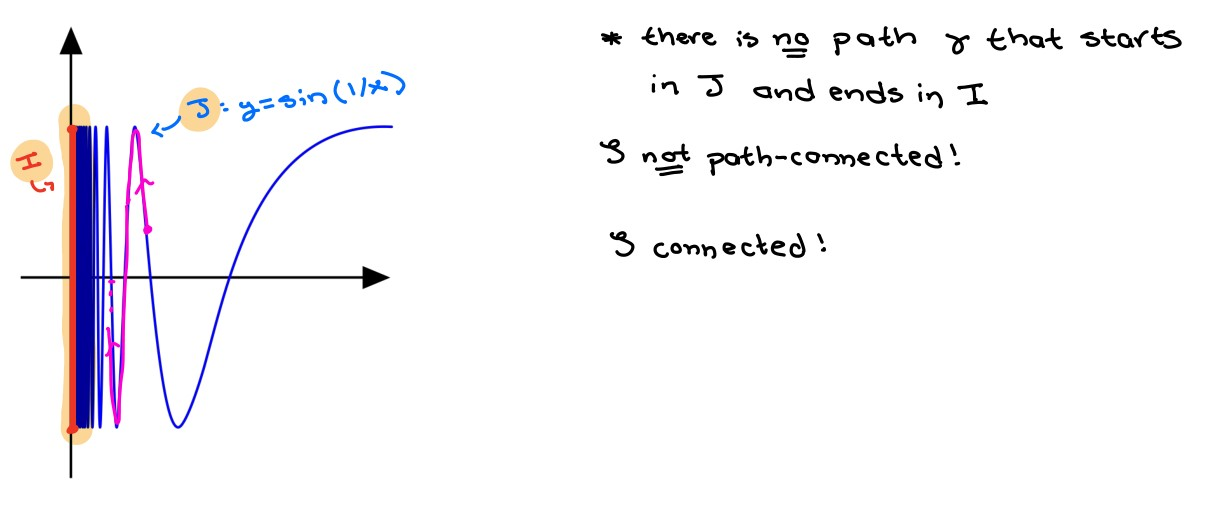
\includegraphics[ width = 0.5\linewidth ]{figures/Section 24/24_eg2.jpg}
        \caption{A visual of the Topologist's Sine Curve}
        \label{fig:24-1}
    \end{figure}
\end{egBox}